% This is part of Un soupçon de mathématique sans être agressif pour autant
% Copyright (c) 2015
%   Laurent Claessens
% See the file fdl-1.3.txt for copying conditions.

\begin{corrige}{2smath-0093}

    Pour cet exercice, il ne suffit pas de répondre qu'on ne peut pas parce qu'on n'a pas la longueur du segment \( [AB]\). En effet, il est demandé de dessiner un triangle \emph{qui respecte tous les codages}, et non qui lit dans les pensées de Anne-Laure. La longueur de \( [AB]\) est donc au choix\footnote{Notons au passage que cette longueur n'est en réalité pas tout à fait au choix parce qu'elle peut se déduire avec Pythagore, mais c'est une autre histoire.}.
    
    La raison de l'impossibilité de dessiner le triangle de Anne-Laure est toute autre. 

        Commençons par donner des noms aux points qui en n'ont pas :

        \begin{center}
        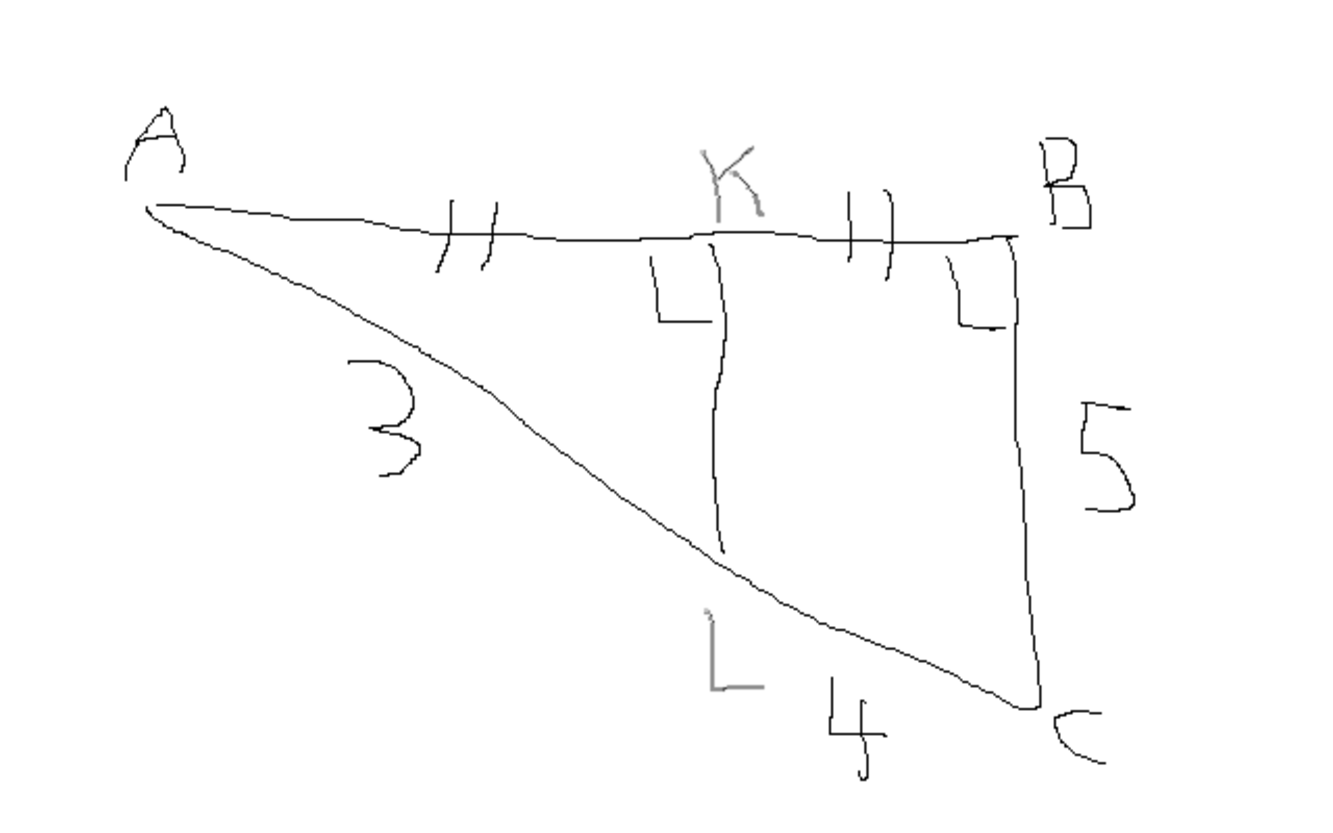
\includegraphics[width=5cm]{faux_triangle_correction.pdf}
        \end{center}

    Le segment \( [KL]\) est parallèle à \( [BC]\) et passe par le milieux de \( [AB]\). Elle est donc une droite des milieux du triangle \( ABC\). Donc \( (KL)\) doit couper \( [AC]\) en son milieu.

    Or les codages indiquent que \( (KL)\) ne coupe pas \( [AC]\) en son milieu (\( 3\) d'un côté et \( 4\) de l'autre). Donc le dessin est impossible.

\end{corrige}
